\chapter{Towards a Citizen Science-Enabled Liquid Democracy Platform}
\label{ch:Approach}
In the previous chapter we provided a theoretical background for citizen science and liquid democracy, showing amongst other things that potential synergies between the two concepts exist.
Therefore, in this chapter we aim to lay the conceptual foundation for a citizen science-enabled liquid democracy platform.
To this end, we will start by deriving a list of criteria such a platform would need to fulfill in \ref{sec:Criteria} before we evaluate existing work based on compliance with these criteria in \ref{sec:RelatedWork}.
Finally, we will present a thorough conceptual sketch of a citizen science-enabled liquid democracy platform in \ref{sec:Conceptual_Approach}.

%nach 3.3
%Thus, this system consists of two core components: (1) a participatory system, which is scaffolding the other core component: (2) an interface allowing interested users to access the system’s data. (1) is describing the concept of liquid democracy and (2) the approach of citizen science.

\section{Criteria}
\label{sec:Criteria}
In this section we want to gather criteria for a \tracknshrink{CS}-enabled \tracknshrink{LD} platform in order to evaluate existing projects on the one hand, and to approach the conceptual design of such a system on the other hand. 
Since we can not enumerate all the possible \tracknshrink{CS} projects with \tracknshrink{LD} backgrounds, we do not think that it is feasible to design a one-fits-all platform.
On the other hand, the \tracknshrink{LD} functionalities of specific platforms can be assumed to not change from project to project.
Therefore, we arrange our criteria in two groups.
Criteria in the first group are directed towards a general \tracknshrink{LD} platform design that can be used in projects both with and without a \tracknshrink{CS} context.
Those in the second group are directed towards a \tracknshrink{CS}-enabling interface a \tracknshrink{LD} platform can implement in order to explicitly support the development of specific \tracknshrink{CS} projects on top of it.

Based on our work in \ref{sec:Liquid_Democracy}, we derive the core functionalities of a \tracknshrink{LD} platform as \textbf{(\tracknshrink{LD}1)} collaborative editing of propositions, \textbf{(\tracknshrink{LD}2)}  secret and verifiable voting on propositions and \textbf{(\tracknshrink{LD}3)} secret and verifiable vote delegation.
We observe that participatory systems on the web tend to produce an overwhelming amount of data and that most modern platforms tackle this problem by content filtering algorithms, which we do not consider to be appropriate for a \tracknshrink{LD} platform due to the danger of censorship.
Rather, we would like to involve the user to actively filter propositions based and therefore derive the fourth criteria for a \tracknshrink{LD} platform as \textbf{(\tracknshrink{LD}4)} active information filtering capabilities.
Furthermore, as each individual in a \tracknshrink{LD} has the right to create propositions, we acknowledge that adversary users could abuse this right to generate a lot of noise (so called spam) in the fashion of a DDoS attack\footnote{\url{https://en.wikipedia.org/wiki/Denial-of-service_attack\#Distributed_DoS}}. Therefore we derive \textbf{(\tracknshrink{LD}5)} implementation of spam prevention mechanisms.
Finally, we derive the last criteria for a \tracknshrink{LD} platform from the discussion in \ref{ssec:Integration_AccessibilityAnonymity} as \textbf{(\tracknshrink{LD}6)} protection of privacy.

We have seen in \ref{sec:Theory_CS} that we can categorize a citizen science project according to the degree of participation and its expected outcome.
Our approach allows the implementation of \tracknshrink{LD}-based \tracknshrink{CS} projects on all levels of Hacklays ladder of participation, since our \tracknshrink{CS}-enabling interface empowers citizen science communities to kickstart their own projects and formulate research questions without the help of professional scientists.
Note that specifically the separation of the \tracknshrink{LD} platform from the \tracknshrink{CS}-enabling interface means that communities could build their \tracknshrink{CS} projects either around existing instances of \tracknshrink{CS}-enabled \tracknshrink{LD} platforms or, if needed, set up their own instance.
The main issue to solve with this interface is the conflict between user privacy, in particular secret voting, and data transparency as layed out in \ref{ssec:Integration_AccessibilityAnonymity}.
For lower levels of participation a more restrictive data access policy could be enforced, while higher levels of participation with involvement of the citizen scientists in the data evaluation and possibly even in the definition of research questions require complete and transparent access to all of the platforms data such as propositions, delegation graphs, voting results etc.
In order to support the highest level of participation possible we see no other way than to trust in the citizen scientists self-responsibility, i.e. to partly relay control over the amount and kind of data shared to the users of the \tracknshrink{LD} platform.
However, as users are not expected to be well trained in privacy protection, the choices of users should not be too fine-grained and rather be envisioned as a number of pre-specified policies.
We therefore derive the additional criteria for a \tracknshrink{CS}-enabling interface as \textbf{(\tracknshrink{CS}1)} default restrictive data access with guaranteed privacy protection and \textbf{(\tracknshrink{CS}2)} opt-in completely transparent data access without guaranteed privacy protection.

\section{Related Work}
\label{sec:RelatedWork}
  
In this section we will explore related projects, that are freely accessible, open source software (\tracknshrink{FOSS}) and which share our two main goals; That is a platform allowing---to some extent---to (1) participate in democratic processes and (2) to access the platform’s data. Therefore, we do not focus on projects that implement regular survey/polling features (e.g., \textit{LimeSurvey}\footnote{\url{https://www.limesurvey.org/}}), as this would be only a small subset of that platform.

Initially, when starting this work in 2017, we discovered some projects that met certain aspects of our main goals. Most of these projects, however, have been (officially) discontinued over time or have not been under active development (no commit for two years or more). Additionally, some of them were commercial projects or closed-source and thus not replicable or adaptable in any way. The website \textit{The Democracy Foundation}\footnote{\url{https://democracy.foundation/similar-projects/}} provides a list ranging from smaller projects to advanced governance platforms. Unfortunately, most of them are outdated as well or are not applicable to our scenario. Nonetheless, there were two potential candidates we took into consideration for building a prototype.

The first promising platform we looked into was \textit{LiquidFeedback}\footnote{\url{https://liquidfeedback.org/}}. It is developed by the \textit{Public Software Group}\footnote{\url{https://www.public-software-group.org/}} and was used by Berlin’s Pirate Party for inner-party decision-making processes. Although the source code is available at the developers’ website, we encountered two major drawbacks. For one, we had difficulties during the setup process\footnote{\url{http://www.public-software-group.org/mercurial/liquid_feedback_frontend/raw-file/tip/INSTALL.html}}, and since there is no developer support (and no official repository, or other public developer community) it is a cumbersome process. Despite being labeled open source it is in the interest of the developer to implement the platform as payed service. Additionally, due to the large usesage of the programming language Lua---where none of us had any prior experience---we decided to skip this project.

The other candidate is \textit{DemocracyOS}\footnote{\url{http://democracyos.org/}}, which is actively developed by Argentina’s Net Party (span. \textit{Partido de la Red}). This platform provides a modern tech stack (backend: MongoDB, frontend: React) and good developer support\footnote{Docs: \url{http://docs.democracyos.org/} GitHub: \url{https://github.com/DemocracyOS/democracyos}}. Unfortunately, the project is structured in an obscure manner; for example the developers decided against differentiating between \texttt{src} files and \texttt{lib} files, thus mixing React components with regular helper functions and other libraries in on big \texttt{lib} folder. Since there is no clear separation of view, logic and helper libraries this creates an entangled graph of dependencies.

Despite both platforms, especially the latter one, are both promising tools, there is still one fundamental issue: As of 2019 there is no \tracknshrink{FOSS} platform that implemented the idea of vote delegation in any way, and does provide sufficient support to engage developers. Since developing our very own digital liquid democracy platform would be an enormous project, we shifted our focus towards a conceptual framework.



% Participedia is a meta website gathering data from other sites:
% \url{https://www.wissenschaftsmanagement.de/news/participedia-demokratie-staerken-durch-geteiltes-wissen-und-bielefelder-forscher-entwickeln}

% nVotes is a simple voting plattform this could also be done with normal survey platforms such as LimeSurvey, so this not taken into account

\section{Conceptual Design}
\label{sec:Conceptual_Approach}
In this section we will develop a conceptual overview of both a \tracknshrink{LD} platform and a \tracknshrink{CS}-enabling interface based on the criteria derived in \ref{sec:Criteria}.
This task will be approached methodically from three conceptual views: data fragments, user roles and processes.
We start by describing different data fragments that occur within a liquid democracy.
%Namely, these are propositions, the centerpiece of democratic discourse: propositions, their properties and lifecycle.
Then we describe the various roles users can take in the platform.
Having a clear view on both data fragments and user roles, we then discuss the core processes of a \tracknshrink{CS}-enabled \tracknshrink{LD} platform.
%Lastly, we elaborate the utility of notifications for a \tracknshrink{LD} platform and illustrate how the \tracknshrink{CS}-enabling interface exhibited by the platform can be used by citizen science projects.

\subsection{Data Fragments}
\label{ssec:data_fragments}
%In this section, we will present the essential data fragments in a \tracknshrink{LD} platform.

\subsubsection{Propositions}
\label{sec:Model_Propositions}
A democracies most important process in order to transform political positions and individual opinions into laws is the iteratively joint crafting of propositions which are, once finalized, subject to voting.
Propositions therefore should be the first thing to think about when developing the concept of a \tracknshrink{LD} platform.
Apart from a title, the proposition text and a list of voting options, propositions possess additional metadata and dependency relationships to other data fragments in the platform.
Metadata is very important for the accessibility of the actual information content, for example through active filtering mechanisms as required by \textbf{(\tracknshrink{LD}4)}.
Amongst others, proposition metadata include proposition creator, time of creation and the political context as well as the administrative unit a proposition belongs to.

By political contexts (from here on just contexts), we mean the categorial themes in which political topics are organized.
The context a proposition is associated with is a crucial piece of metadata in a \tracknshrink{LD} platform, as  clearly defined categories are important to make order of the ongoing topics and are essential to stay on top of things.
As with most categorial organization systems, broad, general contexts can be divided down to narrower, more specficic ones and thus form a taxonomy, which we will discuss in detail in~\ref{sec:Model_Contexts}.

Propositions typically evolve over time which can be conceptualized as a succession of versioned snapshot.
To this end, a propositions state should be saved together with an increasing version numer at either fixed time intervals or manually by the individuals involved with the editing.
Moreover, a propositions creation and its evolution should always be accompanied by a healthy discussion of the matter at hand between both individuals directly involved with the proposition editing and other individuals interested in expressing their political opinions.
These discussions contents and their metadata are discussed in the next section.

\subsubsection{Discussion Entries}
\label{ssec:Discussion_Entries}
Discussion entries are posts from users that can be attached to several other data fragments that allow discussion.
To allow an efficient evaluation of participants opinions on the direction of the discourse, discussion entries can be up- or downvoted by other users.
Additionally, the textual content of a discussion entry can carry hyperlinks to a selection of other data fragments that it references.
Examples of data fragments that should be referencable by hyperlinks in discussion entries are propositions, proposition change requests and discussion entries themselves.

\subsubsection{Proposition Change Requests}
\label{ssec:Proposition_Change_Requests}
As we discussed briefly in the previous section about propositions, a proposition will evolve over its life time which means that it will be edited.
Since it is desirable that edits to propositions are funded on a discursive process involving multiple individuals as required by \textbf{(\tracknshrink{LD}1)} we argue that only the original creator of the proposition, i.e. its owner, should be able to directly edit it.
In order to allow other individuals to support the editing process, we introduce proposition change requests, which are data fragments that carry the edited propositon text together with a linked discussion entry and a reference to the underlying proposition. 
These proposition change requests can then be accepted or rejected by the owner of the proposition.
In addition to up- or downvoting the linked discussion entry, users can explicitly express their conditional support of the proposition in case the proposition change request gets accepted or rejected.
This should help the responsible proposition owners to determine the value of specific change requests.
Proposition change requests should not be used to completely turn a propositions goal on its head.
For these cases there exists alternative propositions which will be discussed next.

\subsubsection{Alternative Propositions and Proposition Groups}
\label{ssec:AltProposition}
In most cases, politics are too complex to capture the endeavor of all individuals in one proposition that can be answered with a simple yes or no.
In order to provide means to depict political opinions more accurately, we introduce alternative propositions.
Alternative propositions have all the properties of normal propositions with the exception that the political contexts of alternative propositions can not be different from those of the original proposition.
Additionally, alternative propositions carry a reference to the original proposition, effectively placing them in a common \emph{proposition group}.

\subsubsection{Context Taxonomy}
\label{sec:Model_Contexts}
While we earlier looked at contexts as metadata of propositions, in order to categorize propositions effectively, a context taxonomy must exist prior to proposition creation, which makes such a taxonomy an independent data fragment.

Choosing a proper context taxonomy to categorize propositions is crucial for a \tracknshrink{LD} project as it is a sort of foundation for the work to follow.
On the one hand the contexts can help users to find votes they are interested in, which partly satisfies criteria \textbf{(\tracknshrink{LD}4)}.
Even more important, with contexts one can also determine for which issues one wants to vote oneself and which topics one wants to pass on to a person with more expertise in this field.
Taking for example a vote about the deforestation of the south of Germany, it could fall into a context such as environment.
Imagining that the someone is not that much of specialist when it comes to the environment and wants to delegate votes for propositions on this subject to a relative who is.
%Here the taxonomies not only determine if he gets the topic in his feed but it also could automatically be passed on to his relative.
%This highlights a second problem: how do we make sure that the votes are categorized properly?
%More about this later.
%First, we have to make sure to set up a fundamental category that covers a wide spectrum of the political issues existing.

In general, a taxonomy for \tracknshrink{LD} propositions should meet three elemental requirements.
First and foremost, the taxonomy must be exhaustive as we want to make sure that every occurring vote is covered.
Secondly the categories need to be disjunct, meaning that two categories shouldn't describe the same subject.
Additionally, the categories should be able to adapt and evolve as the political landscape as well changes with time.
A taxonomy that fulfills all requirements perfectly probably does not exist, but we tried to find one already existing system that met our requirements as best as possible.

A well-known external and source for document categorization is the Wikipedia taxonomy.
The corpus of the open encyclopedia is often used to build automatic categorization approaches or to improve the performance of existing models.
Seeing the pure size of the corpus and the fact that it changes constantly you don’t wonder why this is the case.
For our project however, the problem occurred that the political category described more the field of political science that general topics politics are coping with. 

Almost the complete opposite was true for the for the taxonomy of Stack Overflow Politics.
While the Wikipedia articles were almost purely about a scientific view on Politics, the branch of the well-known question and answer site Stack Overflow almost only consist of current topics discussed by the community.
The created tags are therefore more useful for characterizing political topics.
But as the issues discussed are tagged by the user posting the question, it often occurs that there are two tags describing the same field.
So, taking the Stack taxonomy would have cost us a lot of time cleaning the data. 

Going on searching for a more organized alternative we considered the taxonomy that classify the topics discussed by the Bundestag.
For every new legislation period the parliament is putting together committees for different topics.
Even if the number and names of these committees have slightly changed over time, the content is more or less consisting.
On the official Website of the Bundestag we found a tabula sorting all protocols of the committees' meetings.
The altogether 43 topics describe a bride range of political topics.
From family to energy the categories are clearly structured, exhaustive and disjunct, therefore covering two of our tree requirements.
Hence, we recommend to use this taxonomy as a starting point for newly created \tracknshrink{LD} platform instances.
We note that in order to meet our third requirement, the platform should possess mechanisms for the collaborative editing of the taxonomy which will be described in section~\ref{ssec:Context_Taxonomy_Evolution}.

\subsubsection{Delegation Graphs}
As we have seen in \ref{sec:Liquid_Democracy}, delegation graphs are directed graphs where vertices represent participants in a liquid democracy and edges represent the flow of votes from a \textit{principal} to a \textit{proxy}.
Although theoretically delegation graphs can contain cycles, these have no practical meaning, because all the votes of the participants involved in cycles will never contibute to final voting results if the cycle remains unbroken.
On the other hand, as soon as one participant in the cycle choses to vote directly, the cycle is broken.
Therefore, for purposes of vote couting, we can always extract an \emph{effective delegation graph} from a given delegation graph by removing all its cycles.
Note that with this model, cycles can be used by groups of participants with considerable overlap in their political opinions to pool their votes, effectively making sure that all their votes will be counted if at least one of them votes directly.

Delegation graphs can be maintained for different levels of governance, hereafter named scopes.
Scopes have increasing priority with descreasing generality.
Delegation graphs with proposition scope have the highest priority and correspond to specific propositions, i.e. for each proposition there can be at most one delegation graph with proposition scope.
Right below proposition scope we have context scope, where for each context there can be at most one delegation graph with context scope.
The quasi ordering induced by the tree-shaped hierarchical context taxonomy can be used to determine a strict ordering between context-scoped delegation graphs with an ancestor relationship.
This means that for two given contexts $c_1$ and $c_2$, where $c_1$ is a supercontext (ancestor) of $c_2$, $\text{prio}(c_2)>\text{prio}(c_1)$ holds.
Finally, the lowest scope on the priority ladder is the global scope and there can be at most one delegation graph with this scope. 

We will see in \todo{@KD: ref einfügen} how priority can be used for vote counting.

For privacy reasons, delegation graphs with global or context scope are not materialized.\todo{@KD: move this to 4 and elaborate}

\subsubsection{User Intents}
\label{ssec:User_Intents}
The next type of data fragment are so called user intents, which are categorized into vote intents and delegation intents.
Delegation intents can be used to compose delegation graphs while vote intents are the digital counterpart of ballots.
In order to meet the requirements of \textbf{(\tracknshrink{LD}2)} and \textbf{(\tracknshrink{LD}3)} user intents should be anonymized to satisfy the secrecy property as well as public and authorized to satisfy the verifiability property.
To this end. user intents should not only carry information about the specific intent but also authorization information.

\subsubsection{User Accounts}
\label{ssec:User_Accounts}
User accounts are an important instrument to build trust amongst users of a \tracknshrink{LD} platform.
They can potentially offer a variety of personal as well as professional and political information about a certain user.
\todo{@KD: haveTime ? elaborate : leaveAsIs }
However, in order to follow the protection of privacy \textbf{(\tracknshrink{LD}6)}, users should be able to chose themselves which information they want to be displayed to the public.
Moreover, as we have seen in the previous section on user intents, user accounts are decoupled from sensitive political information, i.e. the user intents by means of anonymization.

\subsubsection{Notifications}
\label{sec:Notifications}
As we already discussed in \ref{sec:Criteria}, information overflow is a problem that needs to be dealt with to ensure the scalability of the platform.
A good way to handle the information distribution within the platform and therefore contribute to meet \textbf{(\tracknshrink{LD}4)} is through notifications.
Notifications are information about the creation of new information relevant to the user, generally due to their role within the political process.
As such, notifications can be realized as messages sent to all 'interested' stakeholders within a process.

%Declaring interest within the system can be modeled through assume a certain role.
%However, notifications also can depend on user-determined settings within the profile, which can filter out certain notifications.
%Since this mechanism is described with the users, the following describes the possible notifications a user can receive.
%Notifications exist for:\todo{@KD:exist sounds like this is discussing the implementation already. better wording to distinguish this as a design?}
%\begin{itemize}
%\item Vote delegation of other users 
%\item For Proposition Followers: when propositions change (text or phase) or relevant discussion entries take place, or when alternative propositions are created
%\item For Proposition Followers: When propositions are voted upon / results on the voting are known
%\item For a Proposition Author: When a proposition change request is created
%\item For a Proposition Author: When a moderator changes the context
%\item For Moderators: When a report (inappropriate context or discussion entry) is filed
%\item For Discussion Participants: When someone responds to the respective entries
%\item For Context Followers: When a proposition in the context of interest is created
%\item For Context Followers: When the context taxonomy changes regarding followed interests
%\item For Delegates: When a delegated vote is withdrawn
%\item For Vote Delegators: When a vote was used in a proposition 
%\end{itemize}
\todo{@KD: move the commented stuff to chapter 4}

\subsubsection{Moderation Requests}
\label{ssec:Moderation_Requests}
Moderation requests are instrumental in enforcing platform rules, as they can help to prevent spam \textbf{(\tracknshrink{LD}5)} as well as other malicious and non-tolerable actions on the platform such as hate speech and advertisement.
Users can issue moderation requests for data fragments that are prone to abuse such as propositions, proposition change requests and discussion entries.
A moderation request carries a reference to another data fragment together with a message that details the specific kind of platform rules violation.
A group of trusted, privileged users can then take action on these requests.

\subsection{User Roles}
\label{sec:UserRoles}
%\todo{how many, what they can do and why}
This section will describe the roles that users on the platform can take on.
It is important to note that this is done from a perspective of what roles different stakeholders take in the relevant processes, and that it takes on the perspective of the business processes.

This is not meant to imply that only some users can take on these roles or that these roles are technically different, and is not meant to restrict access to processes.
We believe, as derived in \ref{sec:Liquid_Democracy} and \ref{sec:Theory_CS} that both from a citizen science as well as from a liquid democracy perspective participation in a democracy should be only as restricted as necessary, and as open as possible.
While we do think that discursive structures need to be established within discussions, the possibilities for participation should not be restricted.

In the following we will describe the roles the political subject can take within the structures of discourse in the platform and we will justify why we think that access to these discursive activities should be limited to users taking on this role in the given context.

\subsubsection{Proposition follower}
A proposition follower is a user that has expressed an interest in a given proposition. Proposition followers will receive updates on the state of a proposition, alternative propositions based on it, changes in wording and contributions to the discussion about the proposition.

This does not grant them any rights any other user does not have, and it is thus simply a conceptual role that needs to be regarded in the notification system.

\subsubsection{Proposition author}
\label{ssec:Roles_propositioner}
The propositioner is the role a user can take on when initiating the political process by starting a \hyperref[sec:Model_Propositions]{proposition}.
%Since the process of propositions is already described in \ref{sec:Model_Propositions}, the following focuses on the role.
A propositioner has the right to change the text of a proposition, either by editing directly, or by moderating the proposition change requests.
Access to these activities is limited to the propositioner in order to guarantee consistency of the proposition, and to incentivize discussion about aspects relevant to users not in the role of the propositioner.
Not allowing other users to edit the proposition also prevents malicious or strategic editing as well as discussions about text changes through change requests.
By having to seek approval for modification, a discourse about the aspects important to the proposition modification requester is strengthened.
Moreover does the proposition editing restriction encourage alternative propositions, strengthening the discourse through (hopefully) constructive alternatives.

As we have seen in \ref{ssec:AltProposition}, users can also create alternative propositions to existing ones, thus becoming alternative proposition authors.
These propositions are assigned to the same proposition group.
For this proposition the alternative proposition author counts as \hyperref[ssec:Roles_propositioner]{proposition author}, and has the same rights as them for the same reasons.
Since an alternative proposition works basically the same way as the original proposition, the differentiation between a proposition author and an alternative proposition author is merely semantical. 

By creating a proposition (or an alternative proposition), a user becomes a proposition follower of this proposition as well.

\subsubsection{Discussion participant}
\label{ssec:Roles_DiscussionParticipant}
As the name suggests, a discussion participant is a user that engages in a discussion about some data fragment by creating a discussion entry.
Users become discussion participants as soon as they contributes to the discussion by writing a discussion post or responding to one.
\todo{@all: decide whether this means that the user receives notifications about the discussion. Also decide whether she becomes a proposition follower through this}.

\subsubsection{Proposition modification requester}
The proposition modification requester is a \hyperref[ssec:Roles_DiscussionParticipant]{discussion participant} that raises a constructive proposition text edit request. 
As noted in \ref{ssec:Proposition_Change_Requests}, a proposition text edit request proposes the addition, deletion or textual editing of a passage of proposition text, with (potential) new wording.

\subsubsection{Moderator}
\label{ssec:Roles_Moderator}
A moderator is a user with a particular interest and reputation in a context (or a number of contexts).
Moderator status can be issued to users that engaged in the platform over a prolonged stretch of time within a given context or a number of its subcontextes, if the user so wishes.
The moderator role gives a user moderating power of the moderation requests falling within the context they moderate, such as deciding whether a users' behavior is inappropriate, posts should be deleted (or at least flagged as questionable) or (in conjunction with moderators of other contexts) whether a user should be (temporally or permanently) banned from the platform.

Whether these actions can be performed by a moderator alone, or require the decision of a ,,moderator counci'' depends on the policy of the are very specific questions that we do not aim to answer in this conceptual platform design.
This also hold for deciding how inappropriate behavior of moderators is dealt with.

Moderators / a council of moderators further decides about changes to the taxonomy regarding the context of their responsibility.
How changes in the taxonomy are managed is described in section~\ref{sec:Model_Contexts}.

\subsubsection{Supporter}
\label{ssec:Roles_Supporter}
A supporter is a user that expresses agreement with a 'discursive entity' in order to provide some assessment about the popularity of contributions to a discussion.
These can come from a large range of sources, such as propositions, proposition change requests or discussion entries. 

%Of these proposition groups, (alternative) propositions in the discussion phase and change requests are crucial for the author of them assess how the political process with these could go.

%In addition to helping the author to assess the political mood, support has some functional aspects as well:
%\begin{itemize}
%\item For a proposition group support decides whether a proposition group enters a discussion phase (see \hyperref[ssec:Lifecycle_Initiation]{proposition initiation phase})
%\item For a proposition in discussion phase support for the original or an alternative proposition (in most cases) decides whether an alternative proposition will enter the voting phase (see \hyperref[ssec:Lifecycle_Discussion]{proposition discussion phase})
%\item For a change request support has no direct functional consequences; An incorporated change request however might however, depending on the configuration, translate directly into support for the changed proposition if the change request supporter (or the respective delegated votes) doesn't yet support the proposition in the discussion phase (\todo[inline]{discuss this}). The support for a change request also sends a strong signal for the proposition initiator for political support of this proposition
%\item While this is not necessarily the case (and might depend on the configuration of the system), support for a discussion entry might add to its relevance, potentially placing it on a more visible spot within he discussion threat. Depending on the operators frontend, the support for a discussion entry assists the ranking of the discussion entry (\todo[inline]{discuss}).
%\end{itemize}

\todo{@KD: reconsider where to put commented stuff (if time)}

\subsubsection{Voting Right Holder}
\label{ssec:Roles_VotingRightHolder}
A voting right holder is any user that is allowed to vote on a proposition.
Since utilizing ones own vote overwrites vote delegation, technically every user is a voting right holder for any proposition; Often time however, a user will not exercise their own voting right after delegating their vote.
In this case the term 'voting right holder' refers to the user the vote is delegated to. 

Unsurprisingly, voting right holder are users that can participate in the voting process of a proposition.

\subsubsection{Delegator}
\label{ssec:Roles_Delegator}
A delegator is a voting right holder that delegated his voting right for a single proposition or a number of propositions falling within the same context.
Although a delegator can use her voting right on any propositions (and basically (temporarily) revoke the delegation) and become a voting right holder again, in the usual case it assumed that the voting right was delegated to not exercise the voting right.
If the voting right was delegated for in context scope, it counts as delegated for all subcontexts and all propositions falling within these bounds. 

\subsubsection{Delegate}
\label{ssec:Roles_Delegate}
A delegate is a user that another user delegated their voting right to.
They thus carry votes with them and can basically decide how the delegator voted for propositions falling within the scope of the vote delegation.
Delegates can further delegate votes delegated to them, transferring their votes and the votes delegated to them to the delegate of their choice. 
hrough this they become a delegator with all that this entails.
Observe that this can be done differently for context as well as proposition scope, making them both delegator and delegate for different delegation scopes.

\subsubsection{Admin}
\label{ssec:Roles_Admin}
The admin(s) of the platform should be appointed by the platforms operator and have the most powerful position within it.
In addition to providing the technical infrastructure of the platform and to be able to change its configuration, they also act as a point of appeal for users that deem the decisions of the moderators as inappropriate, and admins can overwrite the decisions of the moderators.
In drastic cases, admins are also authorized to revoke the status of moderators if repeated inappropriate behavior has been reported. 

Administrators have a unique standing in the roles of the platform, in that they are not users, and are thus left outside of the political process, ensuring their neutrality in the discourse.

\subsection{Processes}

\subsubsection{Life Cycle of Propositions}
\label{ssec:Model_Propositions_Life}
\todo{@KD:check}
\begin{figure}[H]
\centering
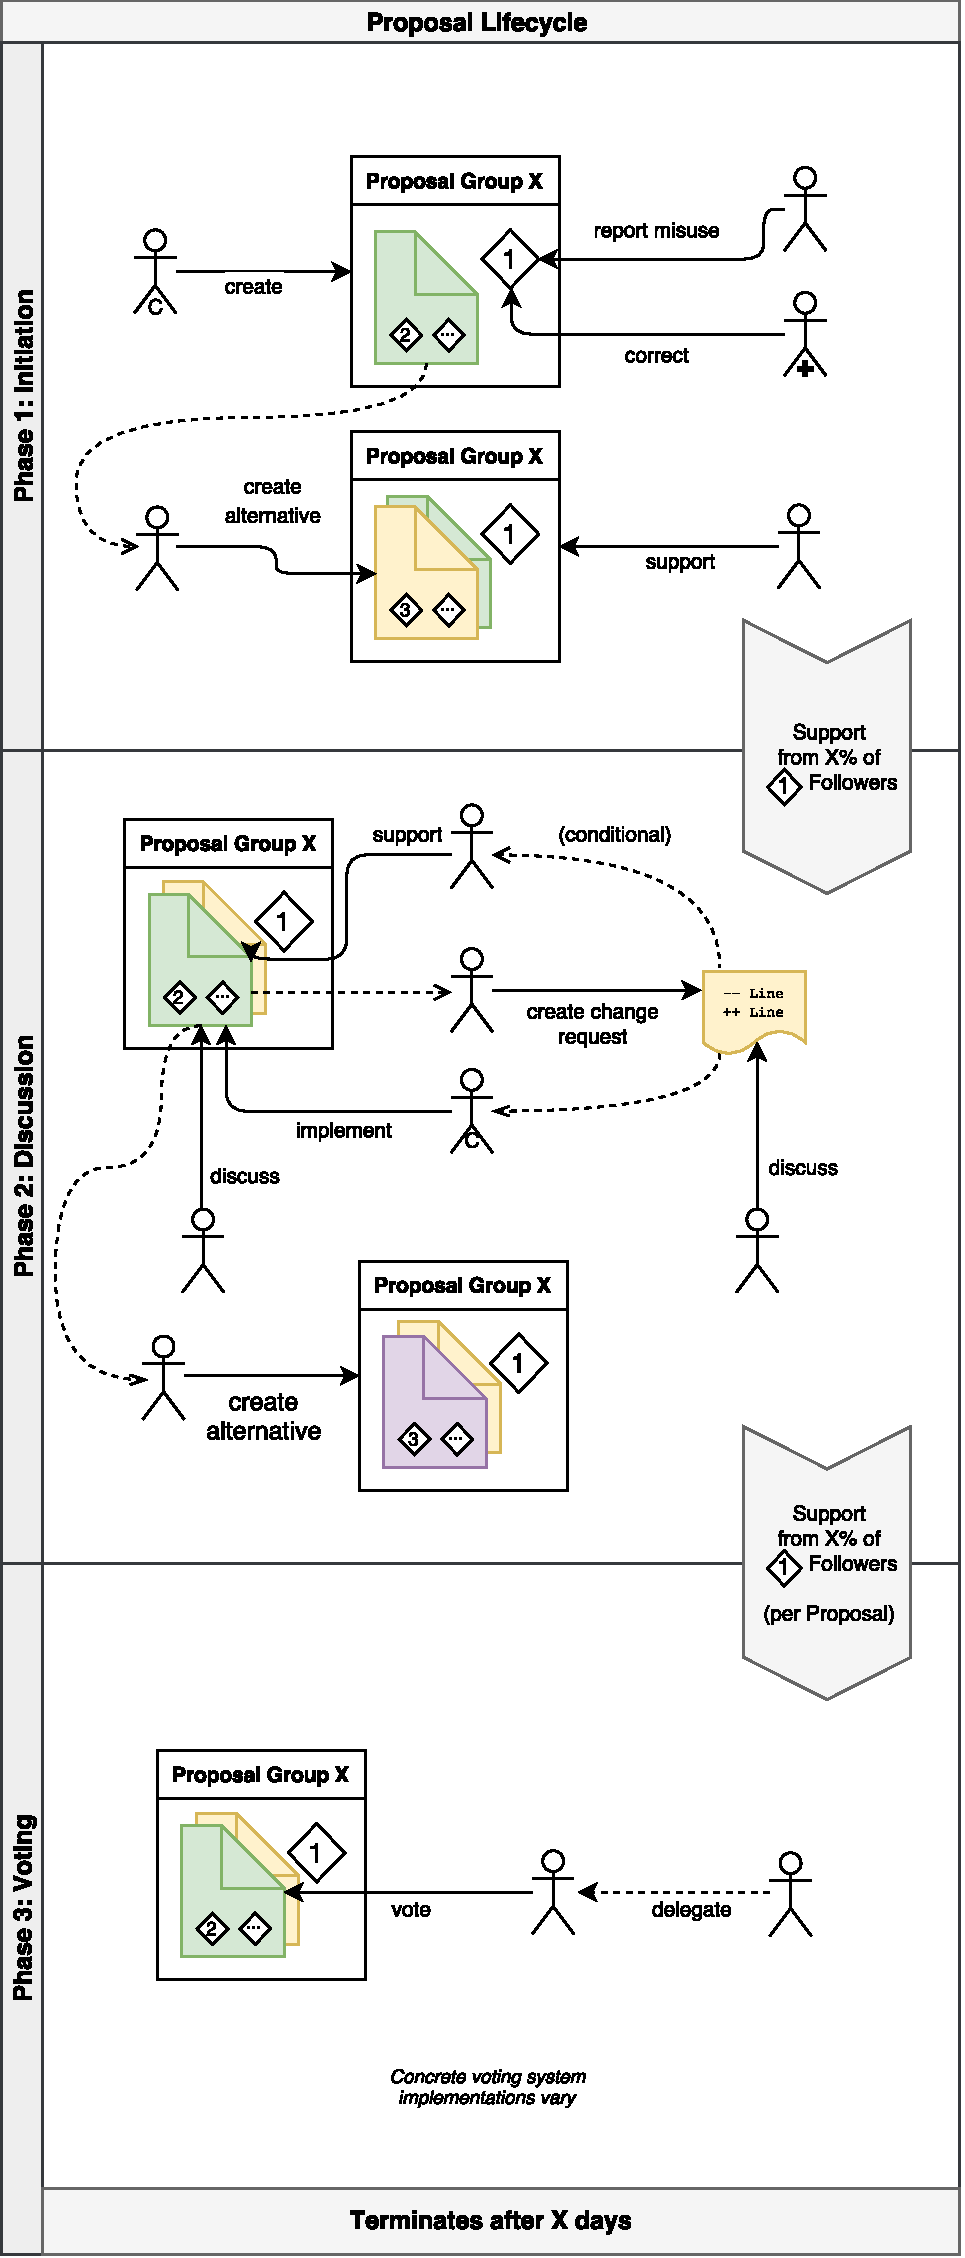
\includegraphics[height=0.6\paperheight]{img/lifecycle_flow_v0.pdf}
\caption{Flow chart of the proposition life cycle}
\label{fig:proplife}
\end{figure}


This process, starting with the initiation of a proposition and ending with the final vote cast, will consequently be dubbed the proposition life cycle.
We split the proposition life cycle into three different phases: (1) initiation, (2) discussion and (3) voting.
It intuitively makes sense to separate a propositions constitutive phase from its voting phase in order to guarantee that the intention of a casted vote stays consistent.
We also subdivide the constitution phase into initiation phase and discussion phase in order to cope with high amounts of individual propositions by allowing only the most appealing propositions to be discussed, thereby channeling the communities efforts and creating an efficient political environment.

In the following, we will successively illustrate each phase by describing its pre- and postconditions as well as its artifacts, actors and their interactions.

\paragraph{Initiation phase}
\label{ssec:Lifecycle_Initiation}

The initiation phase begins when a new proposition is created by an user, which thereby becomes its proposition author (see \ref{ssec:Roles_propositioner}).
To create a proposition, the proposition author needs to specify the following mandatory information: a title, a main text, one primary context, any number of secondary contexts and any number of voting options.
When a new proposition is created, it gets assigned to a new unique proposition group and we call it that proposition groups \emph{root proposition}.
Other users can then create alternative propositions which share the same proposition group, title and primary context as the root proposition.
Creators of alternative propositions are called alternative proposition authors.
Proposition authors, as well as alternative proposition authors can always edit their respective propositions text, options and secondary contexts.
Followers of a proposition groups primary context that are interested in getting it into the discussion phase can attest their support.
Once a proposition group gains enough support ($X\%$ of the primary context follower population), all propositions in it are moved into the discussion phase.

%As the primary context 

\paragraph{Discussion phase}
\label{ssec:Lifecycle_Discussion}

When moving into the discussion phase, more interactions between the supporters and the proposition authors are enabled while all interactions from the initiation phase are maintained.
Users may now issue proposition modification requests to the texts.
Moreover, as previously described in~\ref{ssec:Proposition_Change_Requests}, users can express support for the proposition under the condition that a given modificiation request gets accepted or rejected.
As another means of community involvement in the proposition constitution, users can discuss a proposition.
In discussion entries, special links can be used to reference other data fragments on the platform.
Referencable data fragments are either other discussion entries, (passages of) propositions or (passages of) modification requests.
Other than in the intiation phase, support is not aggregated per proposal group.
Once a single proposition gains enough support ($X\%$ of the primary context follower population), it is moved into the voting phase.

\paragraph{Voting phase}
\label{ssec:Lifecycle_Voting}
The voting phase is very different from the two previous phases, as entering it means all abilities to edit the proposition are revoked.
Discussions are still enabled as we do not want to restrict freedom of expression.
With the beginning of the voting phase legitimated users are able to either delegate their vote or place it on their own.
The voting phase ends after a set amount of days that should be specified by the platform admins.
All user intents that are voiced after the voting phase ends are not considered valid.
A detailed description of the voting mechanism is given in the following section.


\subsubsection{Voting}
\label{sec:Voting_Mechanism}
\todo{@KD:refactor}

%Traditionally, in a parliamentarian democracy, the right to initiate and vote on propositions is exclusive for members of the parliament.
%However, in a liquid democracy every citizen has the right to vote on propositions and to participate in their constitutive phase. Consequently, every participant should also have the unrestrained right to create propositions.
%In an anonymized large-scale digital liquid democracy, this right could be abused by malicious users to mass-create spam propositions in order to bury other propositions for example.
%This threat could be tackled by (1) phased proposition life cycles, (2) adaptive sorting algorithms based on bayesian filtering and (3) moderation.
%Moreover, a strategy may involve that a user cannot create more than \textit{n} proposition per month/year.
%The value \textit{n} needs to be carefully chosen, either it is static hard-coded for all citizens or it is dynamically chosen by a citizen’s trustworthiness.

% \todo[inline]{move implementation-specific details to \ref{sec:Implementation_Voting} and keep this description conceptual}

In order for the voting mechanism to fulfill the criteria developed in \ref{sec:Criteria}, the voting mechanism has to be secret, verifiable and decentralized.
Ideally, it shouldn't be possible for any actor in the system to gather any information about the voting behavior of a voter, while at the same time being verifiable for any actor that votes got counted correctly. 

In line with the principles of security-by-design, in the following we will describe a design for vote casting and counting mechanism that allows manipulation-resistant secret vote casting, which largely preserves privacy.
While not being ideal, due to our lack of expertise in zero-knowledge-proof designed systems, the mechanisms described in the following fulfills these criteria well enough for a prototype.
The main feature of our system design is that both votes and delegations are casted publicly, i.e. it is distributed over the Internet in a way that (1) everyone can access them and (b) no non-critical number of malicious users is able to take down votes.
That means that votes may be casted using a distributed ledger, a publicly managed collection of mirrored vote servers or any other system that abides by these criteria.
Given there is a way to obtain the power of a vote and to verify the vote is valid, casting votes in a public space gives everyone the ability to count and verify votes.
To this end our system requires one central trusted authority: the voting registry (VR), which  contributes to the verifiability of the process by providing means of identifying a given vote as valid.
This is done using a cryptographic method known as blind signature.
The argument for introducing a centralized service into the system is that in any democratic environment some authority has to decide who is part of that environment and therefore has the right to vote.
Note that by using a blind signature scheme secrecy is preserved because the central authority has no ability to link a given vote to an identity.
The vote has been \emph{blindly} singed, i.e. no information about what was signed has been retained. 
Surely, one could imagine a system where the right to vote is granted based on consensus, especially in rather small democratic environments.
However, as we are not familiar with the field, we are not aware if it can be mathematically proven that such a system can work at any scale and have thus decided to not follow this idea.

For a given user and a proposition, the vote casting mechanism works as follows:
\begin{enumerate}
\item The user creates a fresh RSA key pair.
The length of the key should be as large as possible to protect against attacks for the foreseeable future.
\item The user authenticates at the vote registry.
\item If the user is authorized to vote, the vote registry blind signs the public key the user has generated in the first step.
\item The user can now announce vote or delegate intents to the public.
To this end, the user assembles the appropriate message and signs it with his private key he generated in the first step.
Then, he adds his public key from the first step and the unblinded signature from the third step to the message.
The whole message is then posted to a public space that abides by the criteria outlined earlier.
\end{enumerate}

%\paragraph*{Remarks}
% \begin{itemize}
% \item 
% \end{itemize}


\subsubsection{Vote Delegation}
\label{sec:Model_VoteDelegation}
\todo{@KD:refactor}
Vote delegation is the process of transferring voting rights for a proposition or a context (or a number of them) to a delegate.
Technically this means that the vote of the delegate is counted several times (once for the delegate as voting right holder and once for each delegation towards him).
From a social perspective this means a transfer of trust from the delegator to the delegate in an area of trust, whether this may be established from expertise, sympathy or other reasons.
As such, the delegation mechanism encompasses attracting support publicly (what would be campaigning for a vote as a candidate in the representative system), friendship, different trust-based mechanisms and much more; These social phenomenon however are not technically relevant for a \tracknshrink{LD} platform and while \nameref{ssec:User_Accounts} provide restriced means of trust mediation, most of these social processes will be external to the platform. 
%The vote delegation can be visualized via a delegation graph (), a directed graph with the users as nodes and the delegations as edges.
%One could either have a distinct delegation graph for every proposition, for every context, or have one delegation graph with an edge for every delegation (i.e. a labeled multigraph). \todo[inline]{This is more implementation than model and should probably be descruibed in ch.\ref{ch:ProjectRequirements}}
%As with Liquid Feedback, this model avoids circular graphs by breaking the loop with the vote of one of the delegators (implicitly revoking the delegation for the respective proposition; see \href{http://principles.liquidfeedback.org/}{the Liquid Feedback book}).

Delegation mechanisms can be used for all stages of the \hyperref[sec:Model_Propositions]{proposition lifecycle}, i.e. for proposition group initiation support, support in the discussion phase and the voting phase.
The decentralized model of publicly stating delegate intents which was already introduced in section~\ref{sec:Voting_Mechanism} can be used throughout all these stages, effectively giving citizen scientists the ability to harvest data about the evolution of the delegation graph from proposition creation to the close of votings.


\subsubsection{Context Taxonomy Evolution}
\label{ssec:Context_Taxonomy_Evolution}
The evolution of the context taxonomy should be a joint effort between users interested in particular contexts and responsible moderators.
Therefore, the platform should allow for discussions on specific contexts.
Whenever an (informal) consensus is reached amongst participants in such an discussions, a couple of responsible moderators should contact the platform administators which can then implement the change.

For reasons of data integrity, changes to the context taxonomy should be very well justified and moderators should in general have rather conservative stances on changing the context taxonomy

We therefore decided to not design specific data fragments and roles to make this process more automatable and independent from the platform administrators.
Another argument for this non-integrative approach is that, depending on the actual platform implementation, it might not be trivial to guarantee data integrity for specific taxonomy changes and hence might require expert knowledge to execute.


%\subsection{Feedback von Stimmendelegation}
% * <johanning@informatik.uni-leipzig.de> 2018-02-12T12:49:41.623Z:
% 
% > \subsection{Feedback von Stimmendelegation}
% > \label{sec:Model_VoteFeedback}
% > Feedback on the delegation of votes is mediated through notifications. 
% > As mentioned in \ref{sec:Notifications}, delegators are notified when their votes are used in a 'relevant' way by the delegate. Relevancy is managed through user profile settings. 
% 
% What was this supposed to be about (unless I was the one putting it in)?
% 
% ^.
%\label{sec:Model_VoteFeedback}
%Feedback on the delegation of votes is mediated through notifications. 
%As mentioned in \ref{sec:Notifications}, delegators are notified when their votes are used in a 'relevant' way by the delegate. Relevancy is managed through user profile settings. 



%
%\subsection{Researchers Access}
%\label{sec:Model_ResearchersAccess}
%% * <johanning@informatik.uni-leipzig.de> 2018-02-12T12:15:14.572Z:
%% 
%% > \subsection{Researchers Access}
%% > \label{sec:Model_ResearchersAccess}
%% 
%% How concrete should we sketch this? Right now its just a 'we need to be aware of this', but I feel it needs to be more concrete...
%% 
%% ^.
%Since this project takes a Citizen Science approach to Liquid Democracy, researchers access to the data generated by the platform is crucial. Discussing this issue depends heavily on how the problem of accessibility and anonymity raised in \ref{ssec:Integration_AccessibilityAnonymity} is handled, since this determines how researchers / citizen scientists can access the data of interest and defines their range of action with the data of the platform. 
%
%\ref{ssec:Integration_AccessibilityAnonymity} mentions four strategies to deal with user data. While most of the approaches described provide a lot of fine-grained data to the researcher over a large number of users, and allow them a large range of research questions to ask, the aggregative approach (and to some degree the selective aggregative and the deflecting responsibility approach) restrict the data available for researchers. 
%
%More important than the availability of the data might be the accessibility of the data. For this it is decisive that APIs for accessing information relevant to researchers are included in the design of the platform. Since in CS, technical proficiency (or its development) can't be expected, one of the requirements of the design of the APIs is that 'relevant' information is readily available for non-professionals, be it through accessible (and thoroughly documented) APIs or frontends that present relevant information.
%
%While this can't be implemented to its fullest within the scope of this project, this aspect needs considerable consideration in the development of the platform (i.e. in ch. \ref{ch:ProjectRequirements}).
%
%%Steven
%\subsection{Visualization of the Processes}
%\label{sec:Model_Visualization}
%
%%Clara, Simon
%\subsection{Citizen Science Lab Processes}
%\label{sec:CSLab_Processes}
%% Prozess vom Lab schildern, also Fragestellung, Datensammeln, Analysieren und Publizieren: Hier einleiten
%
%%darstellen wie wiss. und nicht-wiss. zusammenarbeiten; inwiefern citizens mÓglichkeit haben in prozess einbezogen zu werden und zu agieren
%
%The workflow of the citizen science lab is sketched in the following.
%
%\subsubsection{Involvement in Formulating Research Questions}
%
%\subsubsection{Citizen Data Collection Process}
%
%\subsubsection{Data Analysis Tools}
%
%\subsubsection{Citizen Science Publication Process}
